\section{Biplots\label{biplot}}

\cite{Chatzipetrou2010} have proposed to use biplot to visualize
the results of CV. Biplot is a way to graphically present data from
two dimensional table. Rows of the table represent samples or individuals
and columns hold different variables. Hence in case of CV results
each row of the table consists of prioritization values assigned by
particular stakeholder and each row corresponds to one prioritization
item.

Biplot consists of rays and dots (see Figure \ref{fig:Biplot-Elements}).
Rays start in center point of biplot, they represent the rows in the
table (i.e. prioritization items). Dots represent rows of the table
(i.e. stakeholders). Links are the lines between the ends of rays.
Table \ref{tab:Interpreting-biplot} lists properties that can be
used to interpret the biplot.

\begin{table}
	\center
	\scriptsize
\caption{\label{tab:Interpreting-biplot}Interpreting biplot}

\begin{tabular}{|>{\centering}p{0.3\textwidth}|>{\centering}p{0.6\textwidth}|}
\hline 
Visual property & Interpretation\tabularnewline
\hline
\hline 
Length of the ray & variation of priority of an item, longer ray represents higher disagreement
between stakeholders on the priority of an item\tabularnewline
\hline 
Distance from a ray to dot & value that stakeholder (represented by the dot) has assigned to the
prioritization item (represented by the ray)\tabularnewline
\hline
Length of the link between the items
& length of link between i1 and i2 is approximately standard deviation of log(i1/i2)\tabularnewline
\hline
The angle between the rays
& cosine of angle between the rays approximates correlation of the corresponding
variables\tabularnewline
\hline 
The distance between the stakeholder dots &
higher distance indicates higher difference between priorities of
stakeholders\tabularnewline
\hline
\end{tabular}
\end{table}

Figure \ref{fig:Biplot-Example-1} shows an example of biplot of the
CV results presented in Table \ref{tab:Data-for-Biplot}. The rows
of the table show priorities assigned by stakeholders (from s1 to
s4) to four prioritization items (from i1 to i4). The variance of
prioritization item i3 is smaller than the variance of i4. That is
displayed in the Figure \ref{fig:Biplot-Example-1} by the fact that
the ray i4 is longer than the ray of i3. If two rays point in the
same direction corresponding variables are positively correlated.
If the angles are negatively correlated the rays point in opposite
directions, i.e. the angle between the rays is close to $180^{0}$.
When the angle is close or equal to $90^{0}$the variables are uncorrelated.
Table \ref{tab:Data-for-Biplot} shows that i3 and i4 are positively
correlated (i.e. when the value of i3 is higher the value of i4 is
also higher and the other way around). Therefore the arrows that represent
i3 and i4 point in the same direction in the Figure \ref{fig:Biplot-Example-1}.
On the other hand when the value of i4 increases the value of i1 is
lower. Therefore prioritization items i4 and i1 are negatively correlated
and they point in different directions in the biplot. There is no
relation between the value of i1 and i2 (they are uncorrelated). That
is indicated by the biplot with straight angle between the rays of
these items.

If two stakeholders assign the same priorities they are displayed
in the same dot. If a stakeholder prefers particular prioritization
item the dot that represents the stakeholder is positioned closer
to that item. Table \ref{tab:Data-for-biplot} and Figure \ref{fig:Biplot-example-2}
show example of stakeholder distribution in a biplot. Stakeholders
s1 and s2 have almost the same priorities therefore they are located
closely. They assign highest priority to item i3 and thus are located
near the ray of item i3. Stakeholder s5 assign equal priorities to
all items therefore he is located near to the center of the biplot.

Biplot is rich tool for discovering relationships between the prioritization
items and stakeholders. But it may become difficult to visually interpret
biplot if it has many prioritization items (more than couple of dozen
items).

\begin{figure}
	\center
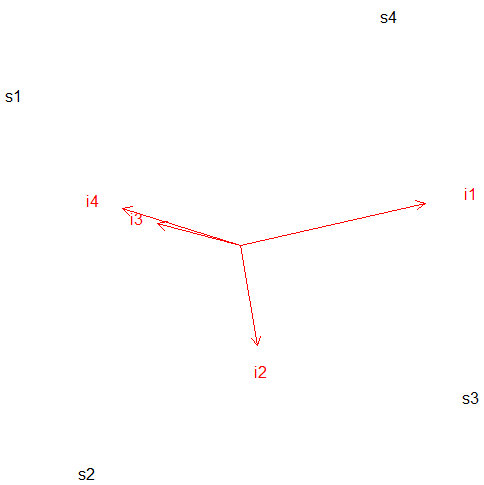
\includegraphics[scale=0.5]{fig/biplot1}
\caption{\label{fig:Biplot-Example-1}Biplot example 1}
\end{figure}

\begin{figure}
	\center
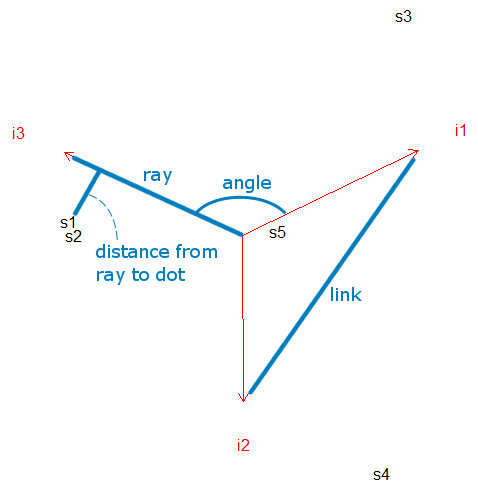
\includegraphics[scale=0.5]{fig/biplot2}
\caption{\label{fig:Biplot-Elements}Biplot elements}
\end{figure}

\begin{table}
	\center
	\scriptsize
\caption{\label{tab:Data-for-Biplot}Data for biplot example 1}
\begin{tabular}{|c|c|c|c|c|}
\hline 
 & \multicolumn{4}{c|}{Prioritization items}\tabularnewline
\hline 
Stakeholders & i1 & i2 & i3 & i4\tabularnewline
\hline
\hline 
s1 & 20 & 20 & 22 & 33\tabularnewline
\hline 
s2 & 20 & 25 & 25 & 30\tabularnewline
\hline 
s3 & 30 & 25 & 20 & 25\tabularnewline
\hline 
s4 & 30 & 20 & 22 & 27\tabularnewline
\hline 
Total priority points for an item & 100 & 90 & 93 & 117\tabularnewline
\hline
\end{tabular}
\end{table}

\begin{table}
	\scriptsize
	\center
\caption{\label{tab:Data-for-biplot}Data for biplot example 2}

\begin{tabular}{|c|c|c|c|}
\hline 
 & \multicolumn{3}{c|}{Prioritization items}\tabularnewline
\hline 
Stakeholders & i1 & i2 & i3\tabularnewline
\hline
\hline 
s1 & 20 & 30 & 50\tabularnewline
\hline 
s2 & 20 & 31 & 49\tabularnewline
\hline 
s3 & 50 & 20 & 30\tabularnewline
\hline 
s4 & 30 & 50 & 20\tabularnewline
\hline 
s5 & 33 & 33 & 34\tabularnewline
\hline 
Total priority points for an item & 153 & 164 & 183\tabularnewline
\hline
\end{tabular}
\end{table}

\begin{figure}
	\center
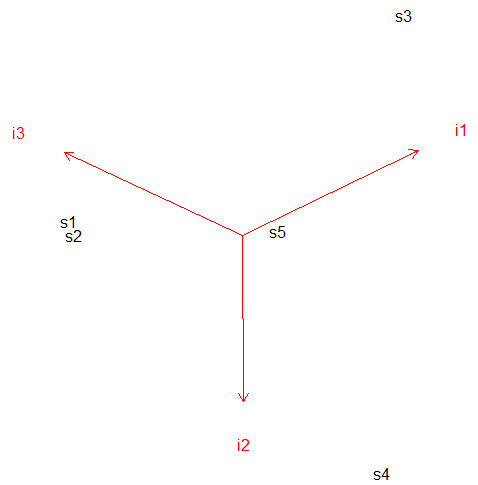
\includegraphics[scale=0.5]{fig/biplot3}
\caption{\label{fig:Biplot-example-2}Biplot example 2}
\end{figure}

\subsection{Drawing biplot}

Creation of biplots for compositional data is described in \cite{Aitchison2002}.
In this chapter we summarize methods that are used to create biplots
in this paper. The methods are implemented in a custom program in
R programming language. The program can be accessed in .

The input for the drawing biplot is $n\times p$ matrix. Matrix has
$n$ rows that represent samples or stakeholders and $p$ columns
that represent variables or prioritization items. Before cumulative
voting results can be plotted they must be transformed using compositional
data analysis. First, zeroes are replaced in the matrix using multiplicative
replacement strategy as described in Section \ref{Problem-of-Zeroes}.
The data is further transformed to create matrix Z. Transformation
is done using logarithmic transformation defined by the equation

\begin{equation}
z_{ij}=\log{}_{e}(x_{ij})-\frac{1}{n}\sum_{k=1}^{p}\log{}_{e}(x_{ik})-\frac{1}{n}\sum_{l=1}^{n}\log{}_{e}(x_{lj})+\frac{1}{n\cdot p}\sum_{m=1}^{n}\sum_{n=1}^{p}\log{}_{e}(x_{lj})\label{eq:biplot}
\end{equation}

where $z$ is the new value of cell in the $i^{th}$ row and $j^{th}$
column, $x$ is the value from cell of initial table.

Next, singular value decomposition (SVD) is calculated from transformed
matrix Z. SVD is a way to divide a matrix into factors that describe
the underlying structure of the matrix. SVD splits matrix Z into three
matrices. By multiplying the matrices are multiplied original matrix
Z can be reconstructed

\begin{equation}
Z=U\Gamma V^{T}\label{eq:SVD}
\end{equation}

U and V are matrices of left and right singular vectors of Z, $\Gamma$is
diagonal matrix $r\times r$ of positive singular values in decreasing
order. U consists of $n\times r$ values and describes the rows of
matrix Z. V consists of $p\times r$ values and describes the columns
of matrix Z. Letter $r$ denotes the rank of matrix Z. Detailed description
on how to perform SVD can be found in \cite{Golub1970}.

In order to construct two dimensional biplot only first two singular
values ($\gamma_{1}$and$\gamma_{2}$), first two left singular vectors
($u_{1}$ and $u_{2}$) and first two right singular vectors ($v_{1}$and$v_{2}$)
are used. Only two values are used because the biplot has only two
dimensions. Therefore the biplot is only approximation of original
matrix Z. SVD ensures that singular values and vectors are ordered
in decreasing order of significance. Hence the first values give
the most information about the original matrix Z. Coordinates of rays
and dots in the biplot are obtained using the following two matrices

\begin{equation}
F=\left[\gamma_{1}^{\alpha}u_{1}\gamma_{2}^{\alpha}u_{2}\right]\, G=\left[\gamma_{1}^{1-\alpha}v_{1}\gamma_{2}^{1-\alpha}v_{2}\right]
\end{equation}

F and G hold first two columns of U and V multiplied by first and
second singular values. Rows of F are used as coordinates for drawing
dots (representing stakeholders) in biplot. Rows of G are used as
coordinates for the end points of the rays of biplot (representing
prioritization items). First column is used for x axis and second
for y axis.

Singular values are powered to $\alpha$ or $1-\alpha$. Alpha can
range from 0 to 1. If $\alpha$ is 1 the biplot is better at showing
relationships between the rows of matrix Z. If the alpha is 0 the
biplot presents the columns better. In this paper we use biplots with
$\alpha$ equal to 0.
